\documentclass{beamer}
\usepackage[utf8]{inputenc}

\usetheme{Madrid}
\usecolortheme{default}
\usepackage{amsmath,amssymb,amsfonts,amsthm}
\usepackage{txfonts}
\usepackage{tkz-euclide}
\usepackage{listings}
\usepackage{adjustbox}
\usepackage{array}
\usepackage{tabularx}
\usepackage{gvv}
\usepackage{lmodern}
\usepackage{circuitikz}
\usepackage{tikz}
\usepackage{graphicx}

\setbeamertemplate{page number in head/foot}[totalframenumber]

\usepackage{tcolorbox}
\tcbuselibrary{minted,breakable,xparse,skins}



\definecolor{bg}{gray}{0.95}
\DeclareTCBListing{mintedbox}{O{}m!O{}}{%
  breakable=true,
  listing engine=minted,
  listing only,
  minted language=#2,
  minted style=default,
  minted options={%
    linenos,
    gobble=0,
    breaklines=true,
    breakafter=,,
    fontsize=\small,
    numbersep=8pt,
    #1},
  boxsep=0pt,
  left skip=0pt,
  right skip=0pt,
  left=25pt,
  right=0pt,
  top=3pt,
  bottom=3pt,
  arc=5pt,
  leftrule=0pt,
  rightrule=0pt,
  bottomrule=2pt,
  toprule=2pt,
  colback=bg,
  colframe=orange!70,
  enhanced,
  overlay={%
    \begin{tcbclipinterior}
    \fill[orange!20!white] (frame.south west) rectangle ([xshift=20pt]frame.north west);
    \end{tcbclipinterior}},
  #3,
}
\lstset{
    language=C,
    basicstyle=\ttfamily\small,
    keywordstyle=\color{blue},
    stringstyle=\color{orange},
    commentstyle=\color{green!60!black},
    numbers=left,
    numberstyle=\tiny\color{gray},
    breaklines=true,
    showstringspaces=false,
}
\begin{document}

\title 
{1.5.21}
\date{August 23,2025}


\author 
{Kavin B-EE25BTECH11033}






\frame{\titlepage}
\begin{frame}{Question}
Find the ratio in which $\vec{P}(4,m)$ divides the line segment joining the points $\vec{A}(2,3)$ and $\vec{B}(6,-3)$. Hence, find $m$.
\end{frame}



\begin{frame}{Theoretical Solution}

Let the vector $\vec{P}$ be 
\begin{align}
    \vec{P}=\begin{myvec}{4\\m}\end{myvec} \;, 
\end{align}
Given the points,
\begin{align}
    \vec{A}=\begin{myvec}{2\\3}\end{myvec}
    \vec{B}=\begin{myvec}{6\\-3}\end{myvec}
\end{align}
The points \vec{A}, \vec{P}, \vec{B} are collinear.\\

\end{frame}

\begin{frame}{Formulae}
\textbf{Points $\vec{A}, \vec{P}, \vec{B}$ are defined to be collinear if}
\begin{align}
		\label{eq:line-rank-2}
		\rank{\myvec{\vec{P}-\vec{A}& \vec{B}-\vec{A}}} = 1
\end{align}
\end{frame}

\begin{frame}{Theoretical Solution}
\begin{align}
            \vec{P}-\vec{A} = \myvec{2\\m-3}\\
            \vec{B}-\vec{A} = \myvec{4\\-6}\\
            \myvec{\vec{P}-\vec{A}& \vec{B}-\vec{A}} = \myvec{2 & 4\\m-3 & -6}
\end{align}
\begin{center}
$R_2 \rightarrow 2R_2 + 3R_1 \implies \myvec{2 & 4\\2m & 0}$
\end{center}
For rank $1$, the second row must be zero:
\begin{align}
    2m=0 \implies m=0
\end{align}
\begin{center}
$\therefore \vec{P}=\begin{myvec}{4\\0}\end{myvec}$
\end{center}
\end{frame}

\begin{frame}{Formulae}
\textbf{Section formula for a vector $\vec{P}$ which divides the line formed by vectors $\vec{A}$ and $\vec{B}$ in the ratio k:1 is given by}
\begin{align}
    \vec{P}=\frac{k\vec{B}+\vec{A}}{k+1}
\end{align}
\begin{align}
			k\brak{\vec{P}-\vec{B}}&= \vec{A}-\vec{P}
\end{align}
\begin{align}
			\implies k &=
			\frac{\brak{\vec{A}-\vec{P}}^{\top}\brak{\vec{P}-\vec{B}}}{\norm{\vec{P}-\vec{B}}^2}
			\label{eq:section_formula-k}
\end{align}
\end{frame}
\begin{frame}{Theoretical Solution}
\begin{align}
\brak{\vec{A}-\vec{P}}^{\top}\brak{\vec{P}-\vec{B}} = \myvec{-2 & 3}\myvec{-2\\3} = 13\\
{\norm{\vec{P}-\vec{B}}^2} = \brak{\sqrt{2^2 + 3^2}}^2 = 13
\end{align}

\begin{align}
\implies k &= 1
\end{align}

Therefore the ratio in which $\vec{P}$ divides the line segment joining the points $\vec{A}$ and $\vec{B}$ is $1:1$\\
\end{frame}


\begin{frame}[fragile]
    \frametitle{C Code - A function to find the value of m}

    \begin{lstlisting}

#include <stdio.h>

float findM(float Ax, float Ay, float Bx, float By, float Px) {
    float k = (Px - Ax) / (Bx - Px);
    float m = (k * By + Ay) / (k + 1);
    return m;
}

    \end{lstlisting}
\end{frame}

\begin{frame}[fragile]
    \frametitle{Python Code}
    \begin{lstlisting}
import numpy as np
import matplotlib.pyplot as plt
import ctypes
import os

c_lib=ctypes.CDLL('./code.so')

# Define the argument types for the findM function
c_lib.findM.argtypes = [ctypes.POINTER(ctypes.c_float), ctypes.POINTER(ctypes.c_float),ctypes.POINTER(ctypes.c_float), ctypes.POINTER(ctypes.c_float),ctypes.POINTER(ctypes.c_float)]
# Define the return type of the findM function
c_lib.findM.restype = ctypes.c_float

    \end{lstlisting}
\end{frame}

\begin{frame}[fragile]
    \frametitle{Python Code}
    \begin{lstlisting}
# --- Define Points and Calculate 'm' using C function ---

# Define the coordinates for the endpoints A and B
A = np.array([2.0, 3.0])
B = np.array([6.0, -3.0])
# Define the known x-coordinate for the dividing point P
Px = 4.0
# Call the C function to get the value of m
m_value = c_lib.findM(
    ctypes.c_float(A[0]), # Ax
    ctypes.c_float(A[1]), # Ay
    ctypes.c_float(B[0]), # Bx
    ctypes.c_float(B[1]), # By
    ctypes.c_float(Px)    # Px
)
    \end{lstlisting}
\end{frame}

\begin{frame}[fragile]
    \frametitle{Python Code}
    \begin{lstlisting}
# Create the dividing point P with the calculated 'm'
P_dividing = np.array([Px, m_value])
def find_ratio(point_A, point_B, dividing_point):
    
    # Ensure all inputs are numpy arrays for vector operations
    A_vec = np.array(point_A)
    B_vec = np.array(point_B)
    P_vec = np.array(dividing_point)
    
    # Calculate the ratio vector. If the points are collinear,
    # the ratio will be consistent for both x and y components.
    # We add a small epsilon to avoid division by zero if P coincides with B.
    epsilon = 1e-9
    ratio_vector = (P_vec - A_vec) / (B_vec - P_vec + epsilon)
    return ratio_vector
    \end{lstlisting}
\end{frame}

\begin{frame}[fragile]
    \frametitle{Python Code}
    \begin{lstlisting}
# Calculate and print the ratio
ratio = find_ratio(A, B, P_dividing)
print(f'Point {tuple(P_dividing)} divides the line AB in the ratio: {ratio[0]}:{ratio[1]}')

def generate_line_segment(point1, point2, num_points=10):
    """Generates points to plot a line segment between two points."""
    dim = point1.shape[0]
    line_segment = np.zeros((dim, num_points))
    lambda_vals = np.linspace(0, 1, num_points)
    for i in range(num_points):
        temp = point1 + lambda_vals[i] * (point2 - point1)
        line_segment[:, i] = temp.T
    return line_segment

# Generate the line segment for plotting
x_AB = generate_line_segment(A, B)
    \end{lstlisting}
\end{frame}
\begin{frame}[fragile]
    \frametitle{Python Code}
    \begin{lstlisting}
# --- Plotting ---
plt.plot(x_AB[0, :], x_AB[1, :], label='$AB$')

# Plot the points A, B, and the dividing point P
all_points = np.vstack((A, B, P_dividing)).T
plt.scatter(all_points[0, :], all_points[1, :])

# Add labels for the points
point_labels = ['A (2,3)', 'B (6,-3)', 'P (4,0)']
for i, txt in enumerate(point_labels):
    plt.annotate(txt, # text to display
                 (all_points[0, i], all_points[1, i]), # point to label
                 textcoords="offset points", # position of the text
                 xytext=(10, 5), # distance from text to points (x,y)
                 ha='center') # horizontal alignment
    \end{lstlisting}
\end{frame}
\begin{frame}[fragile]
    \frametitle{Python Code}
    \begin{lstlisting}
# Set plot details
plt.xlabel('$x$')
plt.ylabel('$y$')
plt.title('Point P(4,0) divides AB in ratio of 1:1')
plt.legend(loc='best')
plt.grid(True)
plt.axis('equal')

# Save the plot to a file
plt.savefig('../figs/fig.png')

# Display the plot
plt.show()
    \end{lstlisting}
\end{frame}


\begin{frame}{Plot}
    \centering
    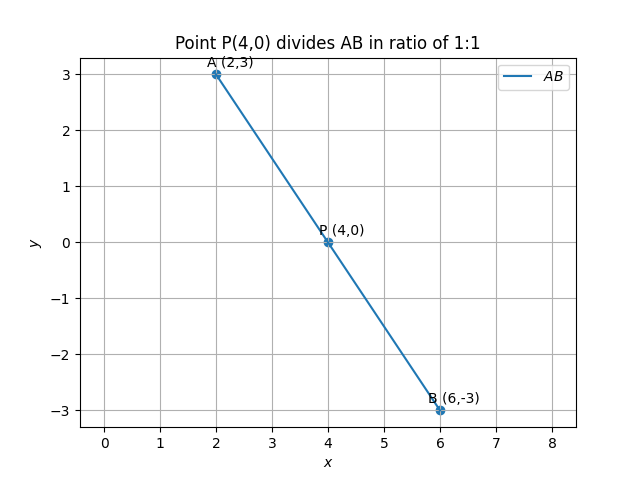
\includegraphics[width=\columnwidth, height=0.8\textheight, keepaspectratio]{figs/fig.png}     
\end{frame}


\end{document}
